\subsection{Discrete Logarithm Problem and Cryptography}
Elliptic and Hyperelliptic curve cryptography are schemes which can be derived from the larger general class of discrete logarithm cryptography schemes. In Whitfield Diffie and Martin Hellman's article: \emph{New directions in Cryptography}~\cite{Diffie:2006:NDC:2263321.2269104} it is described how we can generate a cryptographic scheme from a discrete logarithm, this section will summarise this. We can define the general discrete logarithm problem as follows: suppose we have a prime $p$, we can create a prime field from this prime by setting the integers modulo $p$ and removing 0: $$\mathbb{Z}_p = \mathbb{Z}_p \setminus \{0\}$$ These types of fields are also typically called Prime Galois Fields and can be denoted as $GF(p)$. We can define a cyclic subgroup from this field: $g \in \mathbb{Z}_p$ which means that we now have a group which we can define an arithmetic function over, and if we repeat that arithmetic function on an element some amount of times, we will return to our original element. Now we can define the discrete logarithm problem: Let $Y = \alpha^X\mod{p},$ for $1 \leq X \leq p-1,$ where $\alpha$ is a fixed primitive element of $GF(p)$. Rearranging this equation, we then have $X = \log_aY\mod{p}$ for $1 \leq Y \leq p-1$, and $X$ can be referred to as the logarithm of $Y$ to the base $\alpha,\mod{p}.$ To calculate $Y$ is easy, and we can use the square and multiply algorithm, which is described in Algorithm \ref{squareandmultiply}.
\begin{algorithm}[!htb]
\textbf{Input:} Element $\alpha$, $X$ \\
\textbf{Output:} Element $Y = \alpha^X\mod p$ 
\caption{Square and Multiply Algorithm}\label{squareandmultiply}
\algrule
\begin{algorithmic}[1]
\Function{F}{$\alpha,X$}
\If{$X = 1$}
\Return $X \mod{p}$
\ElsIf{$X\mod{2} = 0$}
\Return $F(\alpha^2\mod{p}, X/2)$ 
\ElsIf{$X\mod{2} = 1$}
\Return $\alpha^2 \times F(\alpha, X-1) \mod{p}$
\EndIf
\EndFunction
\end{algorithmic}
\end{algorithm}
This takes at most $2\log_2p$ multiplications to calculate~\cite{10007220734}. For example for $X = 18$, we have $$Y = \alpha^{18} = (((\alpha^2)^2)^2)^2 \times \alpha^2$$ It is very hard to calculate $X$ given $Y$ however, and for carefully chosen values of $p$, requires on the order of $p^{1/2}$ operations using the best known algorithm~\cite{mcclellan1974art}. 
We can turn this one way function into a cryptographic scheme as follows: We have two parties, Alice and Bob and they agree publicly on a value for $g$, an element from a prime group of size $p$. This element $g$ is known as the generator. Alice picks a random element $a$ and sends to Bob $g^a\mod{p}$. Bob does the same for some random element $b$ : $g^b\mod{p}$. Alice then computes $(g^b)^a\mod{p} = g^{ab}\mod{p}$, and Bob computes $(g^a)^b\mod{p} = g^{ab}\mod{p}$. Now both parties have a shared secret. If some attacker Eve wants to find $a$, $b$ or $g^{ab}\mod{p}$ from $g^a\mod{p}$ and $g^b\mod{p}$, she will have to solve a discrete logarithm problem. This scheme is called Discrete Logarithm Diffie Hellman, and is used to set up a secure communication channel between two parties. There are many more schemes we can derive from discrete logarithm problems, such as certificate generation and verification.  The next sections will describe how we can use elliptic and hyperelliptic curves to define a group which we can then define a discrete logarithm problem over.
\subsection{Elliptic Curve Cryptography}
To begin understanding Hyperelliptic Curve Cryptography, it may be of help to briefly describe Elliptic Curve Cryptography (ECC). An elliptic curve is a set of points that satisfy an equation in the form: $y^2 = x^3 + ax + b$. This type of equation is called a Weierstrass equation. The elliptic curve must also be non-singular, which means that the curve has no cusps, self-intersections or isolated points. A cusp is where a function's gradient becomes infinitely large before returning back on itself, an example of this is shown in Figure \ref{fig:cusp}.
\begin{figure}[!htb]
\centering
\resizebox{5cm}{!}{\begin{tikzpicture}
\pgfplotsset{ticks=none}
\begin{axis}[
        xmin=-4,xmax=5,
        ymin=-5,ymax=5,
        xlabel={$x$},
        ylabel={$y$},
        scale only axis, axis lines=middle,
        domain=-2.279018:3,
        samples=201,smooth,clip=false,
        axis equal image=true
    ]
\addplot[red] {sqrt(x^3)};
\addplot[red] {-sqrt(x^3)};
\end{axis}
\end{tikzpicture}}
\caption{Example of cusp on graph $y^2 = x^3$}
\label{fig:cusp}
\end{figure}
These properties can be achieved algebraically by making sure that the discriminant of the curve is not equal to 0: $$\Delta = -16(4a^3+27b^2) \neq 0$$ Elliptic curves over $\mathbb{R}$ generally look similar to the one in Figure \ref{fig:ECC}.
\begin{figure}[!htb]
\centering
\resizebox{5cm}{!}{\begin{tikzpicture}
\pgfplotsset{ticks=none}
\begin{axis}[
        xmin=-4,xmax=5,
        ymin=-5,ymax=5,
        xlabel={$x$},
        ylabel={$y$},
        scale only axis, axis lines=middle,
        domain=-2.279018:3,
        samples=201,smooth,clip=false,
        axis equal image=true
    ]
\addplot[red] {sqrt(x^3-3*x+5)};
\addplot[red] {-sqrt(x^3-3*x+5)};
\end{axis}
\end{tikzpicture}}
\caption{Elliptic Curve satisfying $y^2=x^3-3x+5$}\label{fig:ECC}
\end{figure}
\subsubsection{Elliptic Curve Arithmetic}
We can "add" two points on an elliptic curve $P$ and $Q$ to give another point $R$ on the curve. This operation is called the dot operation. We can show this operation visually by drawing a straight line through points $P$ and $Q$, and where this line meets the curve again, will be the "inverse" of the result of our dot operation, $R'$. To get $R$, we can draw a vertical line and take the point where this line meets the curve. This process is described in figure \ref{fig:ECCdot}.
\begin{figure}[!htb]
\centering
\resizebox{5cm}{!}{\begin{tikzpicture}
\pgfplotsset{ticks=none}
\begin{axis}[
        xmin=-4,xmax=5,
        ymin=-5,ymax=5,
        xlabel={$x$},
        ylabel={$y$},
        scale only axis, axis lines=middle,
        domain=-2.279018:3,
        samples=201,smooth,clip=false,
        axis equal image=true
    ]
\addplot[red] {sqrt(x^3-3*x+5)};
\addplot[red] {-sqrt(x^3-3*x+5)};
\draw [] (-2.213,0.893) -- (2.264,3.132);
\draw [dashed] (2.264,3.132) -- (2.264,-3.132);
\draw [fill=black] (-2.213,0.893) circle (1pt);
\draw [color=black] (-2.213,0.893) node [left]{$P$};
\draw [fill=black] (0.2,2.1) circle (1pt);
\draw [color=black] (0.2,2.1) node [above]{$Q$};
\draw [color=black] (2.264,3.132) node [right]{$R'$};
\draw [fill=black] (2.264,-3.132) circle (1pt);
\draw [color=black] (2.264,-3.132) node [right]{$R$};
\end{axis}
\end{tikzpicture}}
\caption{Dot operation on two points $P$ and $Q$ to give final point $R$}
\label{fig:ECCdot}
\end{figure}
We can then dot $P$ and $R$ using the same method as before to give us another point on the curve, $S$, as shown in figure \ref{fig:ECCdot2}.
\begin{figure}[!htb]
\centering
\resizebox{5cm}{!}{\begin{tikzpicture}
\pgfplotsset{ticks=none}
\begin{axis}[
        xmin=-4,xmax=5,
        ymin=-5,ymax=5,
        xlabel={$x$},
        ylabel={$y$},
        scale only axis, axis lines=middle,
        domain=-2.279018:3,
        samples=201,smooth,clip=false,
        axis equal image=true
    ]
\addplot[red] {sqrt(x^3-3*x+5)};
\addplot[red] {-sqrt(x^3-3*x+5)};
\draw [] (0.758, -1.778) -- (2.264,-3.132);
\draw [dashed] (0.758, -1.778) -- (0.758, 1.778);
\draw [dashed] (0.758, -1.778) -- (-2.213,0.893);
\draw [fill=black] (-2.213,0.893) circle (1pt);
\draw [color=black] (-2.213,0.893) node [left]{$P$};
\draw [fill=black] (2.264,-3.132) circle (1pt);
\draw [color=black] (2.264,-3.132) node [right]{$R$};
\draw [fill=black] (0.758, -1.778) circle (1pt);
\draw [color=black] (0.758, -1.778) node [below]{$S'$};
\draw [fill=black] (0.758, 1.778)  circle (1pt);
\draw [color=black] (0.758, 1.778) node [above]{$S$};
\end{axis}
\end{tikzpicture}}
\caption{Dot operation on points $R$ and $P$ to give final point $S$}
\label{fig:ECCdot2}
\end{figure}
For our cryptographic function we also need one more operation, point doubling. Point doubling can be achieved by drawing the tangent of the curve at a point $P$, and similarly to point addition, where this tangent intersects the curve will be the inverse of our final point, $Q'$. To get our final point we draw a vertical line and where this line intersects the curve will be our final point $Q$. This process is shown in figure \ref{fig:ECCdbl}.
\begin{figure}[!htb]
\centering
\resizebox{5cm}{!}{\begin{tikzpicture}
\pgfplotsset{ticks=none}
\begin{axis}[
        xmin=-4,xmax=5,
        ymin=-5,ymax=5,
        xlabel={$x$},
        ylabel={$y$},
        scale only axis, axis lines=middle,
        domain=-2.279018:3,
        samples=201,smooth,clip=false,
        axis equal image=true
    ]
\addplot[red] {sqrt(x^3-3*x+5)};
\addplot[red] {-sqrt(x^3-3*x+5)};
\addplot[black] {0.2518*x + 2.924};
\draw [fill=black] (-1.2,2.621) circle (1pt);
\draw [color=black] (-1.2,2.621) node [above]{$P$};
\draw [fill=black] (2.463,3.544) circle (1pt);
\draw [color=black] (2.463,3.544) node [above]{$Q'$};
\draw [dashed] (2.463,3.544) -- (2.463,-3.544);
\draw [fill=black] (2.463,-3.544) circle (1pt);
\draw [color=black] (2.463,-3.544) node [right]{$Q$};
\end{axis}
\end{tikzpicture}}
\caption{Point doubling operation on point $P$ to give point $Q = 2*P$}
\label{fig:ECCdbl}
\end{figure}
\subsubsection{Adapting Elliptic Curve Arithmetic into a Cryptographic Function}
In order to turn our arithmetic into a cryptographic function we must firstly restrict our infinitely many points to a subset of points which is finite. This gives rise to the idea of elliptic curves over finite fields. Particularly useful Galois Fields for our goal of creating a cryptographic function are prime fields of order p and binary extension fields, which can be represented as GF(p) and GF($2^m$) respectively. GF(p) has a prime number of elements equal to p which can be represented as integers, and GF($2^m$) has $2^m$ elements which can be represented as polynomials. Fields of the form GF($2^m$) are particularly useful from a hardware perspective, as elements of the field can be represented as binary strings. For example, the element $x^3 + x + 1$ can be represented in binary as 1011, with each bit corresponding to a coefficient of the polynomial. The set of points of an elliptic curve over a finite field is the set of points in that finite field that satisfy the equation of the elliptic curve. Figure \ref{fig:ECCFF} shows our elliptic curve when it is restricted to elements of the finite field GF(97), it does not resemble our previous curve at all, this is because only the points that hit whole number coordinates are displayed, and the points whose coordinates exceed our prime (97) are wrapped around, e.g. 100 would become 100 mod 97 = 3.
\begin{figure}[!htb]
\centering
\resizebox{5cm}{!}{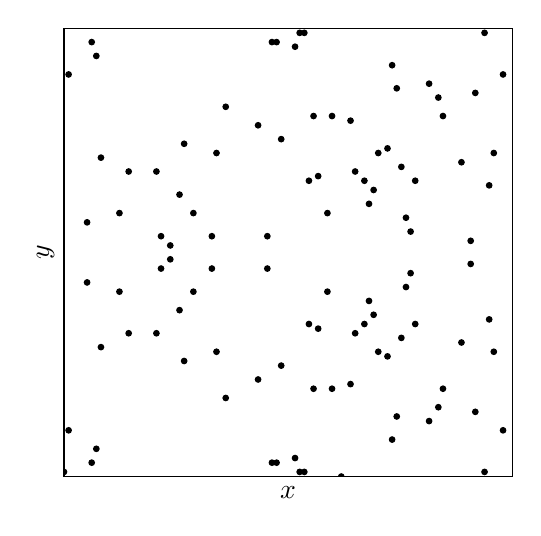
\begin{tikzpicture}
\pgfplotsset{ticks=none}
\begin{axis}[
        xmin=0,xmax=97,
        ymin=0,ymax=97,
        xlabel={$x$},
        ylabel={$y$},
        axis equal image=true
    ]
\draw[fill=black] (0, 1) circle (1pt);
\draw[fill=black] (1, 10) circle (1pt);
\draw[fill=black] (1, 87) circle (1pt);
\draw[fill=black] (5, 42) circle (1pt);
\draw[fill=black] (5, 55) circle (1pt);
\draw[fill=black] (6, 3) circle (1pt);
\draw[fill=black] (6, 94) circle (1pt);
\draw[fill=black] (7, 6) circle (1pt);
\draw[fill=black] (7, 91) circle (1pt);
\draw[fill=black] (8, 28) circle (1pt);
\draw[fill=black] (8, 69) circle (1pt);
\draw[fill=black] (12, 40) circle (1pt);
\draw[fill=black] (12, 57) circle (1pt);
\draw[fill=black] (14, 31) circle (1pt);
\draw[fill=black] (14, 66) circle (1pt);
\draw[fill=black] (20, 31) circle (1pt);
\draw[fill=black] (20, 66) circle (1pt);
\draw[fill=black] (21, 45) circle (1pt);
\draw[fill=black] (21, 52) circle (1pt);
\draw[fill=black] (23, 47) circle (1pt);
\draw[fill=black] (23, 50) circle (1pt);
\draw[fill=black] (25, 36) circle (1pt);
\draw[fill=black] (25, 61) circle (1pt);
\draw[fill=black] (26, 25) circle (1pt);
\draw[fill=black] (26, 72) circle (1pt);
\draw[fill=black] (28, 40) circle (1pt);
\draw[fill=black] (28, 57) circle (1pt);
\draw[fill=black] (32, 45) circle (1pt);
\draw[fill=black] (32, 52) circle (1pt);
\draw[fill=black] (33, 27) circle (1pt);
\draw[fill=black] (33, 70) circle (1pt);
\draw[fill=black] (35, 17) circle (1pt);
\draw[fill=black] (35, 80) circle (1pt);
\draw[fill=black] (42, 21) circle (1pt);
\draw[fill=black] (42, 76) circle (1pt);
\draw[fill=black] (44, 45) circle (1pt);
\draw[fill=black] (44, 52) circle (1pt);
\draw[fill=black] (45, 3) circle (1pt);
\draw[fill=black] (45, 94) circle (1pt);
\draw[fill=black] (46, 3) circle (1pt);
\draw[fill=black] (46, 94) circle (1pt);
\draw[fill=black] (47, 24) circle (1pt);
\draw[fill=black] (47, 73) circle (1pt);
\draw[fill=black] (50, 4) circle (1pt);
\draw[fill=black] (50, 93) circle (1pt);
\draw[fill=black] (51, 1) circle (1pt);
\draw[fill=black] (51, 96) circle (1pt);
\draw[fill=black] (52, 1) circle (1pt);
\draw[fill=black] (52, 96) circle (1pt);
\draw[fill=black] (53, 33) circle (1pt);
\draw[fill=black] (53, 64) circle (1pt);
\draw[fill=black] (54, 19) circle (1pt);
\draw[fill=black] (54, 78) circle (1pt);
\draw[fill=black] (55, 32) circle (1pt);
\draw[fill=black] (55, 65) circle (1pt);
\draw[fill=black] (57, 40) circle (1pt);
\draw[fill=black] (57, 57) circle (1pt);
\draw[fill=black] (58, 19) circle (1pt);
\draw[fill=black] (58, 78) circle (1pt);
\draw[fill=black] (60, 0) circle (1pt);
\draw[fill=black] (62, 20) circle (1pt);
\draw[fill=black] (62, 77) circle (1pt);
\draw[fill=black] (63, 31) circle (1pt);
\draw[fill=black] (63, 66) circle (1pt);
\draw[fill=black] (65, 33) circle (1pt);
\draw[fill=black] (65, 64) circle (1pt);
\draw[fill=black] (66, 38) circle (1pt);
\draw[fill=black] (66, 59) circle (1pt);
\draw[fill=black] (67, 35) circle (1pt);
\draw[fill=black] (67, 62) circle (1pt);
\draw[fill=black] (68, 27) circle (1pt);
\draw[fill=black] (68, 70) circle (1pt);
\draw[fill=black] (70, 26) circle (1pt);
\draw[fill=black] (70, 71) circle (1pt);
\draw[fill=black] (71, 8) circle (1pt);
\draw[fill=black] (71, 89) circle (1pt);
\draw[fill=black] (72, 13) circle (1pt);
\draw[fill=black] (72, 84) circle (1pt);
\draw[fill=black] (73, 30) circle (1pt);
\draw[fill=black] (73, 67) circle (1pt);
\draw[fill=black] (74, 41) circle (1pt);
\draw[fill=black] (74, 56) circle (1pt);
\draw[fill=black] (75, 44) circle (1pt);
\draw[fill=black] (75, 53) circle (1pt);
\draw[fill=black] (76, 33) circle (1pt);
\draw[fill=black] (76, 64) circle (1pt);
\draw[fill=black] (79, 12) circle (1pt);
\draw[fill=black] (79, 85) circle (1pt);
\draw[fill=black] (81, 15) circle (1pt);
\draw[fill=black] (81, 82) circle (1pt);
\draw[fill=black] (82, 19) circle (1pt);
\draw[fill=black] (82, 78) circle (1pt);
\draw[fill=black] (86, 29) circle (1pt);
\draw[fill=black] (86, 68) circle (1pt);
\draw[fill=black] (88, 46) circle (1pt);
\draw[fill=black] (88, 51) circle (1pt);
\draw[fill=black] (89, 14) circle (1pt);
\draw[fill=black] (89, 83) circle (1pt);
\draw[fill=black] (91, 1) circle (1pt);
\draw[fill=black] (91, 96) circle (1pt);
\draw[fill=black] (92, 34) circle (1pt);
\draw[fill=black] (92, 63) circle (1pt);
\draw[fill=black] (93, 27) circle (1pt);
\draw[fill=black] (93, 70) circle (1pt);
\draw[fill=black] (95, 10) circle (1pt);
\draw[fill=black] (95, 87) circle (1pt);
\end{axis}
\end{tikzpicture}}
\caption{The elliptic curve $y^2=x^3-3x+5$ restricted to elements of the finite field GF(97)}
\label{fig:ECCFF}
\end{figure}
With this representation of the elliptic curve, we can also visually show how we can perform arithmetic on points on the curve - to add points, we draw a straight line between the points and when this line hits the "edge", it overlaps continuing from the opposite edge. The point that this line intersects will be the inverse result of adding our two points, so we again draw a vertical line and take the inverse to get our result. This process is shown in figure \ref{fig:ECCFFdot}.
\begin{figure}[!htb]
\centering
\resizebox{5cm}{!}{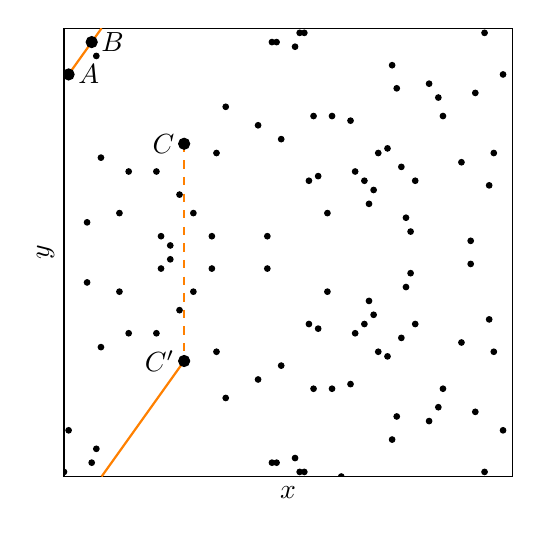
\begin{tikzpicture}
\pgfplotsset{ticks=none}
\begin{axis}[
        xmin=0,xmax=97,
        ymin=0,ymax=97,
        xlabel={$x$},
        ylabel={$y$},
        axis equal image=true
    ]
\draw[orange, thick] (1,87) -- (8.143,97);
\draw[orange, thick] (26,25) -- (8.143,0);
\draw[dashed, orange, thick] (26,72) -- (26,25);
\draw[fill=black] (0, 1) circle (1pt);
\draw[fill=black] (1, 10) circle (1pt);
\draw[fill=black] (1, 87) circle (2pt);
\draw[fill=black] (1, 87) node[right] {$A$};
\draw[fill=black] (5, 42) circle (1pt);
\draw[fill=black] (5, 55) circle (1pt);
\draw[fill=black] (6, 3) circle (1pt);
\draw[fill=black] (6, 94) circle (2pt);
\draw[fill=black] (6, 94) node[right] {$B$};
\draw[fill=black] (7, 6) circle (1pt);
\draw[fill=black] (7, 91) circle (1pt);
\draw[fill=black] (8, 28) circle (1pt);
\draw[fill=black] (8, 69) circle (1pt);
\draw[fill=black] (12, 40) circle (1pt);
\draw[fill=black] (12, 57) circle (1pt);
\draw[fill=black] (14, 31) circle (1pt);
\draw[fill=black] (14, 66) circle (1pt);
\draw[fill=black] (20, 31) circle (1pt);
\draw[fill=black] (20, 66) circle (1pt);
\draw[fill=black] (21, 45) circle (1pt);
\draw[fill=black] (21, 52) circle (1pt);
\draw[fill=black] (23, 47) circle (1pt);
\draw[fill=black] (23, 50) circle (1pt);
\draw[fill=black] (25, 36) circle (1pt);
\draw[fill=black] (25, 61) circle (1pt);
\draw[fill=black] (26, 25) circle (2pt);
\draw[fill=black] (26, 25) node[left] {$C'$};
\draw[fill=black] (26, 72) circle (2pt);
\draw[fill=black] (26, 72) node[left] {$C$};
\draw[fill=black] (28, 40) circle (1pt);
\draw[fill=black] (28, 57) circle (1pt);
\draw[fill=black] (32, 45) circle (1pt);
\draw[fill=black] (32, 52) circle (1pt);
\draw[fill=black] (33, 27) circle (1pt);
\draw[fill=black] (33, 70) circle (1pt);
\draw[fill=black] (35, 17) circle (1pt);
\draw[fill=black] (35, 80) circle (1pt);
\draw[fill=black] (42, 21) circle (1pt);
\draw[fill=black] (42, 76) circle (1pt);
\draw[fill=black] (44, 45) circle (1pt);
\draw[fill=black] (44, 52) circle (1pt);
\draw[fill=black] (45, 3) circle (1pt);
\draw[fill=black] (45, 94) circle (1pt);
\draw[fill=black] (46, 3) circle (1pt);
\draw[fill=black] (46, 94) circle (1pt);
\draw[fill=black] (47, 24) circle (1pt);
\draw[fill=black] (47, 73) circle (1pt);
\draw[fill=black] (50, 4) circle (1pt);
\draw[fill=black] (50, 93) circle (1pt);
\draw[fill=black] (51, 1) circle (1pt);
\draw[fill=black] (51, 96) circle (1pt);
\draw[fill=black] (52, 1) circle (1pt);
\draw[fill=black] (52, 96) circle (1pt);
\draw[fill=black] (53, 33) circle (1pt);
\draw[fill=black] (53, 64) circle (1pt);
\draw[fill=black] (54, 19) circle (1pt);
\draw[fill=black] (54, 78) circle (1pt);
\draw[fill=black] (55, 32) circle (1pt);
\draw[fill=black] (55, 65) circle (1pt);
\draw[fill=black] (57, 40) circle (1pt);
\draw[fill=black] (57, 57) circle (1pt);
\draw[fill=black] (58, 19) circle (1pt);
\draw[fill=black] (58, 78) circle (1pt);
\draw[fill=black] (60, 0) circle (1pt);
\draw[fill=black] (62, 20) circle (1pt);
\draw[fill=black] (62, 77) circle (1pt);
\draw[fill=black] (63, 31) circle (1pt);
\draw[fill=black] (63, 66) circle (1pt);
\draw[fill=black] (65, 33) circle (1pt);
\draw[fill=black] (65, 64) circle (1pt);
\draw[fill=black] (66, 38) circle (1pt);
\draw[fill=black] (66, 59) circle (1pt);
\draw[fill=black] (67, 35) circle (1pt);
\draw[fill=black] (67, 62) circle (1pt);
\draw[fill=black] (68, 27) circle (1pt);
\draw[fill=black] (68, 70) circle (1pt);
\draw[fill=black] (70, 26) circle (1pt);
\draw[fill=black] (70, 71) circle (1pt);
\draw[fill=black] (71, 8) circle (1pt);
\draw[fill=black] (71, 89) circle (1pt);
\draw[fill=black] (72, 13) circle (1pt);
\draw[fill=black] (72, 84) circle (1pt);
\draw[fill=black] (73, 30) circle (1pt);
\draw[fill=black] (73, 67) circle (1pt);
\draw[fill=black] (74, 41) circle (1pt);
\draw[fill=black] (74, 56) circle (1pt);
\draw[fill=black] (75, 44) circle (1pt);
\draw[fill=black] (75, 53) circle (1pt);
\draw[fill=black] (76, 33) circle (1pt);
\draw[fill=black] (76, 64) circle (1pt);
\draw[fill=black] (79, 12) circle (1pt);
\draw[fill=black] (79, 85) circle (1pt);
\draw[fill=black] (81, 15) circle (1pt);
\draw[fill=black] (81, 82) circle (1pt);
\draw[fill=black] (82, 19) circle (1pt);
\draw[fill=black] (82, 78) circle (1pt);
\draw[fill=black] (86, 29) circle (1pt);
\draw[fill=black] (86, 68) circle (1pt);
\draw[fill=black] (88, 46) circle (1pt);
\draw[fill=black] (88, 51) circle (1pt);
\draw[fill=black] (89, 14) circle (1pt);
\draw[fill=black] (89, 83) circle (1pt);
\draw[fill=black] (91, 1) circle (1pt);
\draw[fill=black] (91, 96) circle (1pt);
\draw[fill=black] (92, 34) circle (1pt);
\draw[fill=black] (92, 63) circle (1pt);
\draw[fill=black] (93, 27) circle (1pt);
\draw[fill=black] (93, 70) circle (1pt);
\draw[fill=black] (95, 10) circle (1pt);
\draw[fill=black] (95, 87) circle (1pt);
\end{axis}
\end{tikzpicture}}
\caption{Dot operation on $A$ and $B$ when restricted to finite field GF(97)}
\label{fig:ECCFFdot}
\end{figure}

Using our point double and point addition arithmetic, we can produce any scalar multiplication of a point on an elliptic curve. There are various algorithms which can produce a scalar multiplication of a point, perhaps the most simple would be the "double and add" algorithm. This algorithm is similar to Algorithm \ref{squareandmultiply} for square and multiply, but we instead perform point doubling and point addition. Algorithm \ref{doubleandadd} shows this process.
\begin{algorithm}[!htb]
\caption{Double and Add Algorithm for Scalar Point Multiplication}\label{doubleandadd}
\textbf{Input:} Point $P$, Integer $m$ \\
\textbf{Output:} Point $Q = [m]P$ 
\algrule
\begin{algorithmic}[1]
\Function{scalar\_multiply}{$P,m$}
\If{n = 1}
\Return P
\ElsIf{$n\mod{2} = 0$}
\Return scalar\_multiply(double\_point(P), n/2)
\ElsIf{$n\mod{2} = 1$}
\Return add\_points(P, scalar\_multiply(P, m-1)
\EndIf
\EndFunction
\end{algorithmic}
\end{algorithm}
Once we have our point $Q = [m]P$, it is thought to be very hard to find $m$ given $Q$. This is the basis of the cryptographic function, called the Elliptic Curve Discrete Logarithm Problem (ECDLP). Currently, the best known classical algorithms to solve ECDLP are exponential in the size of the input parameters~\cite{Galbraith2016}. 
The advantages of ECC over commonly used cryptography scheme RSA are that a shorter key can be used whilst keeping the same level of security. We can also generate keys and signatures faster, as well as verifying signatures faster~\cite{gura2004comparing}. This allows for us to generate same levels of security with less hardware, making ECC a good candidate for encryption in cloud services, phones, smart cards, where hardware is at a premium.
\begin{table}[!htb]
\centering
\begin{tabular}{|l|l|l|}
\hline
Symmetric & ECC & RSA \\ \hline
80 & 163 & 1024 \\ \hline
112 & 233 & 2240 \\ \hline
128 & 283 & 3072 \\ \hline
192 & 409 & 7680 \\ \hline
256 & 571 & 15360 \\ \hline
\end{tabular}
\caption{Key lengths needed for equivalent security in ECC and RSA~\cite{gura2004comparing}}
\end{table}
\subsection{Hyperelliptic Curve Cryptography}
While elliptic curves are a subset of hyperelliptic curves with genus equal to 1. A hyperelliptic curve of genus greater than 1 can be formally defined as a curve which satisfies the equation $y^2 + h(x)y = f(x)$ subject to some constraints on $h(x)$ and $f(x)$. The function $f(x)$ is a monic polynomial, the degree of which determines the genus $g$ of the curve. The degree of $f(x)$ can split hyperelliptic curves into two main categories: real hyperelliptic curves and imaginary hyperelliptic curves. When the degree of f(x), $d$ is equal to $2g + 1$, then the curve obtained is said to be imaginary. A degree of $2g+2$ gives a real hyperelliptic curve. This project will focus on imaginary hyperelliptic curves, as these can be developed into a cryptographic function. We can see that our definition of elliptic curves obeys this definition, as an elliptic curve is a hyperelliptic curve of genus 1, and the defining function of elliptic curves must be a monic polynomial of degree 3. The function $h(x)$ is a polynomial of degree less than $g+2$, if the characteristic of the field that the hyperelliptic curve is defined over is not equal to 2, then $h(x) = 0$. Similarly to elliptic curves, the field that the hyperelliptic curve is defined over greatly affects the efficiency of performing arithmetic on the curve. In practice, fields of characteristic 2 have been proven to be the most efficient fields to implement arithmetic over~\cite{gaudry2009arithmetic}. Along with these restrictions, we also require the curve to have no singular points, in the same way that elliptic curves must be. If we view a hyperelliptic curve as lying in the projective plane, $\mathbb{P}^2(K)$, with coordinates $(X,Y,Z)$, then there is a particular point on the curve, known as the point at infinity: $\textit{O} = (0,1,0)$. We can define the opposite of a point $P = (x,y)$ as $\Bar{P} = (x, -y-h(x))$. Figure \ref{fig:HECC} shows a typical imaginary hyperelliptic curve over the real numbers.
\begin{figure}[!htb]
\centering
\resizebox{5cm}{!}{\begin{tikzpicture}
\pgfplotsset{ticks=none}
\begin{axis}[
        xmin=-5,xmax=5,
        ymin=-15,ymax=15,
        unit vector ratio={3 1},
        xlabel={$x$},
        ylabel={$y$},
        scale only axis, axis lines=middle,
        domain=-2.279018:3,
        samples=201,smooth,clip=false,
    ]
\addplot[red, domain=-3:-1] {sqrt(x^5-2*x^4-13*x^3+14*x^2+24*x)};
\addplot[red, domain=-3:-1] {-sqrt(x^5-2*x^4-13*x^3+14*x^2+24*x)};
\addplot[red, domain=0:2] {sqrt(x^5-2*x^4-13*x^3+14*x^2+24*x)};
\addplot[red, domain=0:2] {-sqrt(x^5-2*x^4-13*x^3+14*x^2+24*x)};
\addplot[red, domain=4:4.484] {sqrt(x^5-2*x^4-13*x^3+14*x^2+24*x)};
\addplot[red, domain=4:4.484] {-sqrt(x^5-2*x^4-13*x^3+14*x^2+24*x)};
\end{axis}
\end{tikzpicture}}
\caption{Hyperelliptic Curve satisfying $y^2=x^5-5x^3+4x+1$}
\label{fig:HECC}
\end{figure}

This section will introduce hyperelliptic curves, their group arithmetic operations and how we can define a cryptographic function from these operations.
\subsubsection{Hyperelliptic Curve Arithmetic}
Unlike elliptic curves, there is no group law arithmetic operation over the points of a hyperelliptic curve, this can be shown by the fact that a straight line through two points on a hyperelliptic curve will not always intercept the curve at one more unique point, in fact, Bézout's theorem states that a straight line and a hyperelliptic curve of genus 2 intersect at 5 seperate points. Instead, we must introduce the notion of a divisor, and the Jacobian of a curve $C$, denoted $J_C$. The laws of arithmetic and notation described in this section have been taken from \emph{Handbook of elliptic and hyperelliptic curve cryptography}~\cite{cohen2005handbook}. A divisor, defined by: $$D = \sum_{P_i\in{C}}n_i[P_i]$$ is a set of points on $C$ with integer coefficients $n_i \in \mathbb{Z}$ which are 0 for almost all $i$. The degree of a divisor, $\deg(D)$, is the sum of its coefficients. The set of divisors over a curve is an Abelian group, denoted by $Div_C $, and the subset of degree 0 divisors is denoted by $Div^0_C$. A function on $C$, denoted as $\phi$, is a rational fraction in the coordinates x and y of a point on $C$. The valuation of a function at a point $C$ is denoted as $v_P(\phi)$. We can then define the divisor of a non-zero function on $C$ as: $$div(\phi)=\sum_{P\in{C}}v_P(\phi),$$ a divisor of this type is known as a principal divisor. The set of functions over $C$ is called the function field of $C$ and is denoted by $K(C)$, from this, we can obtain the group of principal divisors of the curve $C$, denoted as $Prin_C$. The set of principal divisors form a subgroup of the group of degree 0 divisors: $$Prin_C \subset Div^0_C$$ Finally, the Jacobian of the curve, denoted as $J_C$, can be defined as the quotient group: $J_C = Div^0_C/Prin_C$. To turn the Jacobian into something we can define a group law arithmetic from, we look at the concept of reduced divisors. A divisor $D$ of $C$ can be called reduced if it has the form $$D = \sum^k_{i=1}[P_i]-k[\textit{O}],$$ where $k \leq g, P_i \neq \textit{O}$. A reduced divisor can be represented by a unique pair of univariate polynomials, conventionally named $u$ and $v$, such that $u$ is monic, and $\deg(v)<\deg(u)\leq g$, this is called the Mumford representation of a reduced divisor, and is very useful for arithmetic purposes. These polynomials take the form: $$u(x) = \sum_{i=1}^r (x-P_i(x)),$$ $$v(P_i(x)) = P_i(y),$$ where $P_i(x)$ and $P_i(y)$ represent the x and y coordinates of point $P_i$ respectively. Therefore, to transform a reduced divisor into its Mumford representation, we first obtain $u$ by setting its roots to the x coordinates of each of the points in the divisor. We can then obtain $v$ as the lowest degree function which passes through each point in the divisor. For genus 2 curves, this is actually quite a simple process: Consider the curve $y^2 = x^5-5x^3+4x+1$ over $\mathbb{R}$, we have two points on this curve: $P_1 = (0,1)$, $P_2 = (1,-1)$. We can define a reduced divisor from these two points as $D = P1 + P2 - 2[\textit{O}]$. Then, we can see that $$u = (x-0)(x-1) = x^2-x,$$ and $$v(0) = 1, v(1) = -1 \therefore v = -2x+1$$
Once we have our reduced divisors in Mumford representation, there are formulae for addition and doubling. The first explicit formula for addition was originally developed by David G. Cantor, hence the name Cantor's algorithm. Cantor's algorithm was further developed by Neal I. Koblitz to look at the general case for curves of any genus. Cantor's algorithm is described in Algorithm \ref{cantor}, originally taken from his paper: \emph{Computing in the Jacobian of a hyperelliptic curve}.~\cite{cantor1987computing}. Cantor's algorithm uses 3 inversions and 70 multiplications, so it has a total complexity of 3I + 70M. Since he first introduced his algorithm, there have been many improvements to the complexity of algorithms for hyperelliptic curve arithmetic, the algorithms which we will use in this project have been taken from \cite{cohen2005handbook}.
\begin{algorithm}[!htb]
\caption{\bf Cantor's Algorithm}
\label{cantor}
\textbf{Input:} Two divisors $\bar{D_1} = [u_1, v_1]$ and $\bar{D_2} = [u_2, v_2]$ on the curve $C : y^2+h(x)y=f(x)$ of genus $g$ \\
\textbf{Output:} The unique reduced divisor D such that $\bar{D} = \bar{D_1}\oplus\bar{D_2}$ 
\algrule
\begin{algorithmic}[1]
\State $d_1 \longleftarrow \gcd(u_1,u_2)$\;
\State $d \longleftarrow \gcd(d_1,v_1 + v_2 + h)$\;
\State $s_1 \longleftarrow c_1e_1, s_2 \longleftarrow c_2e_2$ and $s_3 \longleftarrow c_2$\;
\State$u \longleftarrow \frac{u_1u_2}{d^2}$ and $v \longleftarrow \frac{s_1u_1v_2 + s_2u_2v_1 + s_3(v_1v_2 + f)}{d}$ $mod$ $u$\;
\State repeat\;
\State \ \ \ $u' \longleftarrow \frac{f-vh-v^2}{u}$ and $v' \longleftarrow (-h-v)$ $mod$ $u'$ \;
\State \ \ \ $u \deg u'$ and $v \longleftarrow v'$\;
\State until $deg(u) \leq g$\;
\State make $u$ monic by dividing through by value of first coefficient\;
\State return $[u,v]$\;
\end{algorithmic}
\end{algorithm}
The addition of two divisors on a hyperelliptic curve can also be visualised: we can define a polynomial function which passes through each of the points in each of the divisors of degree $d$, and this line will intersect the curve in exactly $d$ more positions, which will be the opposites of our points which make up our final divisor, similar to the straight line analogy for elliptic curve arithmetic. This process is shown in figure \ref{fig:HECCdot}.
\begin{figure}[!htb]
\centering
\resizebox{5cm}{!}{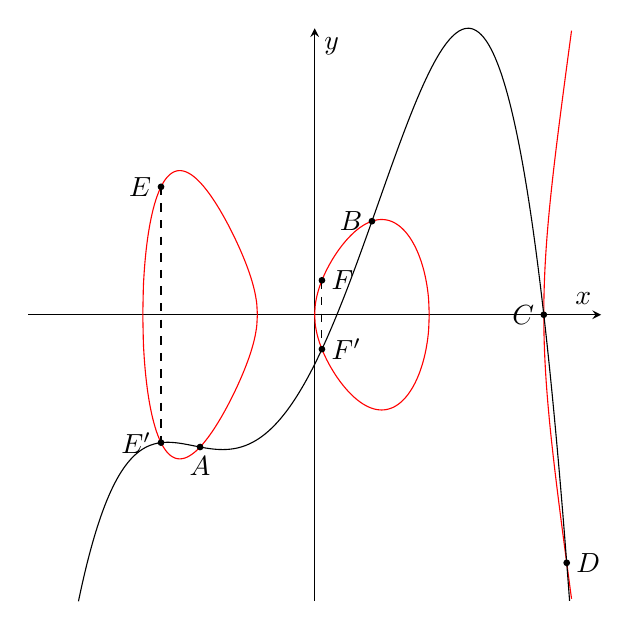
\begin{tikzpicture}
\pgfplotsset{ticks=none}
\begin{axis}[
        xmin=-5,xmax=5,
        ymin=-15,ymax=15,
        unit vector ratio={3 1},
        xlabel={$x$},
        ylabel={$y$},
        scale only axis, axis lines=middle,
        domain=-2.279018:3,
        samples=201,smooth,clip=false,
    ]
\addplot[red, domain=-3:-1] {sqrt(x^5-2*x^4-13*x^3+14*x^2+24*x)};
\addplot[red, domain=-3:-1] {-sqrt(x^5-2*x^4-13*x^3+14*x^2+24*x)};
\addplot[red, domain=0:2] {sqrt(x^5-2*x^4-13*x^3+14*x^2+24*x)};
\addplot[red, domain=0:2] {-sqrt(x^5-2*x^4-13*x^3+14*x^2+24*x)};
\addplot[red, domain=4:4.484] {sqrt(x^5-2*x^4-13*x^3+14*x^2+24*x)};
\addplot[red, domain=4:4.484] {-sqrt(x^5-2*x^4-13*x^3+14*x^2+24*x)};
\addplot[black, domain=-4.123:4.45] {-0.135479279399*x^4-0.269857841745*x^3+1.91253148281*x^2+5.98710284966*x-2.59531772575};
\draw[fill=black] (-2, -6.92820323028) circle (1pt);
\draw[fill=black] (-2, -6.92820323028) node[below] {$A$};
\draw[fill=black] (1, 4.89897948557) circle (1pt);
\draw[fill=black] (1, 4.89897948557) node[left] {$B$};
\draw[fill=black] (4, 0) circle (1pt);
\draw[fill=black] (4, 0) node[left] {$C$};
\draw[fill=black] (4.4, -12.9919605911) circle (1pt);
\draw[fill=black] (4.4, -12.9919605911) node[right] {$D$};
\draw[fill=black] (-2.682, -6.699) circle (1pt);
\draw[fill=black] (-2.682, -6.699) node[left] {$E'$};
\draw[fill=black] (0.127,-1.803) circle (1pt);
\draw[fill=black] (0.127,-1.803) node[right] {$F'$};
\draw[fill=black] (-2.682, 6.699) circle (1pt);
\draw[fill=black] (-2.682, 6.699) node[left] {$E$};
\draw[fill=black] (0.127,1.803) circle (1pt);
\draw[fill=black] (0.127,1.803) node[right] {$F$};
\draw[dashed] (0.127,1.803) -- (0.127,-1.803);
\draw[dashed] (-2.682, 6.699) -- (-2.682, -6.699);
\end{axis}
\end{tikzpicture}}
\caption{Visual representation of adding two reduced divisors: $(A+B) \oplus (C+D) = (E+F)$}
\label{fig:HECCdot}
\end{figure}
\subsubsection{Adapting Hyperelliptic Curve Arithmetic into a Cryptographic Function}
Hyperelliptic curve arithmetic can be adapted into a cryptography scheme in a similar way that elliptic curve arithmetic can, since the set of reduced divisors which make up the Jacobian of the curve form a cyclic group. First, we choose a finite field to define the curve over, typical choices for fields are binary fields and prime fields. Then we can generate a key pair by selecting an initial divisor $D_1 \in J_C$, and each party generating a random integer $k$, which we will use as a scalar multiplier to get a second divisor $D_2$. The key pair will then be $(k, D_2)$ for each party.
\subsubsection{Performance of Hyperelliptic Curve Cryptosystems}
A genus $g$ hyperelliptic curve will have roughly $q^g$ points, where $q$ denotes the number of elements in the field that the Jacobian is defined over. This means when we have a larger genus, we can reduce the size of the field and keep the same levels of security because the order of the group will remain the same. There have been various studies into the performance of hyperelliptic curves against elliptic curves, the main obstacle facing hyperelliptic curve cryptography is the complex nature of the operations required. Table 5 from \cite{pelzl2003hyperelliptic} shows the performance of standard hyperelliptic curves compared to standard elliptic curves, with the hyperelliptic curves of genus 2 being a factor of 1.5 slower than elliptic curves. However, there have been more recent studies such as~\cite{cryptoeprint:2012:670} which suggests implementations of genus 2 curves using Kummer surfaces that can outperform standard NIST elliptic and hyperelliptic curves. Another advantage that hyperelliptic curves have is that the operand length for operations is half (or less) than that of elliptic curves due to the fields being smaller. This means that systems with less complex processors with low or constrained power sources such as those used in many devices in the field of mobile and ubiquitous computing can use hyperelliptic curve cryptography to provide a high level of security.
\subsection{Attacks against Discrete Logarithm Cryptography}
There are various classical attacks against all forms of discrete logarithm problem cryptographic functions. One such attack is called the "Pohlig-Hellman" attack, and essentially reduces the group into smaller prime subgroups, this is why often a prime group is used to define the scheme over, as the group cannot be reduced into smaller subgroups, however it is sufficient to use a group that has a large prime factorisation, so that if someone were to reduce the group, they would still reach a large prime subgroup. Pohlig-Hellman can be used in conjunction with Pollard's rho algorithm for computing discrete logarithms to obtain an attack against the cryptography system which has a run time of $\textit{O}(\sqrt{p}),$ with $p$ being the largest prime factor of the group which the scheme is defined over. For this reason, we must choose a sufficiently large $p$ so that this attack becomes infeasible. This prime $p$, is used to define the key size, denoted by $\lceil \log p \rceil $. The key size determines the security of a discrete logarithm cryptographic system, as well as the running time of encryption and decryption, so we do not want it to be too large as that will affect the speeds that we can encrypt and decrypt at. Another attack specifically against hyperelliptic curve cryptography is the "index calculus algorithm", which becomes more efficient than Pollard's rho method when the genus of the curve is too large. This algorithm has a running time of $\textit{O}(q^{2-\frac{2}{g}+\in})$ where $g$ is the genus of the curve~\cite{theriault2003index}. For this reason, the genus of a curve is suggested to be less than 3 to ensure security against this attack~\cite{scholten2003introduction}.